\documentclass[border=10pt]{standalone}
\usepackage{tikz}
\usetikzlibrary{math, intersections}
\begin{document}
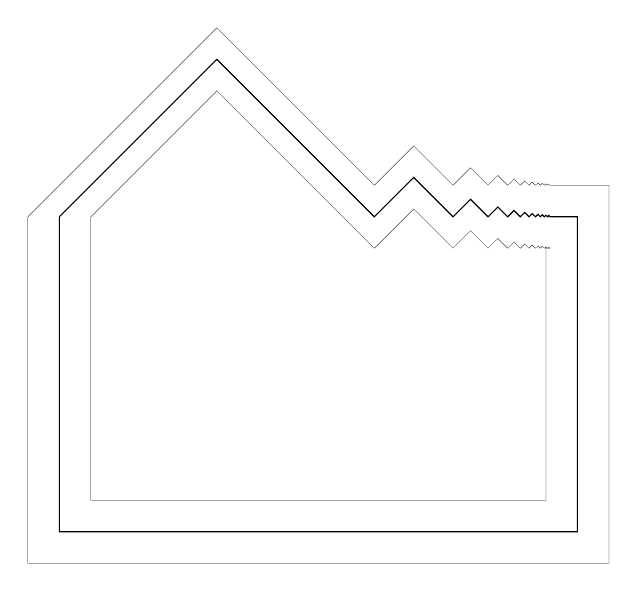
\begin{tikzpicture}
  \pgfmathsetmacro{\scale}{4}
  \pgfmathsetmacro{\numiter}{10}
  \tikzmath{
    function harm(\n) {
      if \n == 0 then{
        return 0;
      } else {
        return \scale/(\n^2) + harm(\n-1);
      };
    };
    function xstart (\n) {
      return harm(\n);
    };
    function xend (\n) {
      return harm(\n+1);
    };
    function xmid (\n) {
      return (xstart(\n)+xend(\n))/2;
    };
    function dx (\n) {
      return (xend(\n)-xstart(\n))/2;
    };
  }

  \pgfmathsetmacro{\xfinal}{\scale*pi^2/6}

  % Draw the core of the neighborhood (the knot)
  \draw (0,0)
  \foreach \n in {0,...,\numiter}{
    -- ({harm(\n)}, 0) -- ({xmid(\n)}, {dx(\n)}) -- ({harm(\n+1)}, 0)
  } -- (\xfinal, 0) -- (\xfinal, -\scale) -- (0, -\scale) -- (0,0);

  \pgfmathsetmacro{\dy}{\scale*.1}

  % Draw the upper boundary for the tubular neighborhood
  % \pgfmathsetmacro{\xbend}{-\dy * sqrt(2)/2}
  % \pgfmathsetmacro{\ybend}{\dy * sqrt(2)/2}
  \draw[ultra thin] (0,\dy)
  \foreach \n in {0,...,\numiter}{
    -- ({harm(\n)}, \dy) -- ({xmid(\n)}, {dx(\n)+\dy}) --
    ({harm(\n+1)}, \dy)
  } -- (\xfinal+\dy, \dy) -- (\xfinal+\dy, -\scale-\dy) -- (-\dy,
  -\scale-\dy) -- (-\dy, 0) -- (0,\dy);



  \draw[ultra thin] (\dy,0) -- ({xmid(0)}, {dx(0)-\dy})
  \foreach \n in {1,...,\numiter}{
    -- ({harm(\n)}, -\dy) -- ({xmid(\n)}, {dx(\n)-\dy}) --
    ({harm(\n+1)}, -\dy)
  } -- (\xfinal-\dy, -\dy) -- (\xfinal-\dy, -\scale+\dy) -- (\dy,
  -\scale+\dy) -- (\dy,0);


\end{tikzpicture}
\end{document}
